\chapter{Giới thiệu}
\label{chap:introduction}

Luận văn này trình bày một framework mã nguồn mở cho phép xây dựng hệ thống nhận dạng hoạt động con người (Human Activity Recognition --- HAR) dựa trên cảm biến quán tính và triển khai kết quả trực tiếp lên vi điều khiển. Trọng tâm của nghiên cứu là giải quyết khoảng cách giữa giai đoạn huấn luyện mô hình trong môi trường Python và giai đoạn suy luận trên thiết bị nhúng tài nguyên hạn chế --- một vấn đề thực tiễn mà các công cụ hiện có chưa xử lý thỏa đáng.

Chương này được tổ chức như sau. Phần~\ref{sec:intro_context} giới thiệu bối cảnh ứng dụng và vai trò của HAR trong hệ sinh thái thiết bị đeo thông minh. Phần~\ref{sec:intro_challenges} phân tích các thách thức kỹ thuật đặc thù của triển khai biên. Phần~\ref{sec:intro_platforms} đánh giá các nền tảng hiện có và xác định khoảng trống nghiên cứu. Phần~\ref{sec:intro_problem} phát biểu bài toán, mục tiêu và đóng góp của luận văn. Các phần cuối trình bày phạm vi và cấu trúc luận văn.

\section{Bối cảnh và động lực nghiên cứu}
\label{sec:intro_context}

\subsection{Thiết bị đeo thông minh và cảm biến quán tính}

Sự tiến bộ của công nghệ vi mạch trong hai thập niên gần đây đã cho phép tích hợp nhiều cảm biến --- gia tốc kế, con quay hồi chuyển, từ kế, cảm biến nhịp tim --- vào các thiết bị đeo nhỏ gọn với chi phí và mức tiêu thụ năng lượng ngày càng thấp. Kết quả là một hệ sinh thái thiết bị đeo phong phú đã hình thành: từ đồng hồ thông minh và vòng tay theo dõi sức khỏe đến miếng dán cảm biến y tế và thiết bị hỗ trợ vận động. Song song với đó, các thuật toán học máy ngày càng hiệu quả đã mở ra khả năng suy luận thông minh ngay trên thiết bị, không cần truyền dữ liệu lên đám mây \cite{warden2019tinyml}.

Trong hệ sinh thái này, \textbf{cảm biến quán tính} (Inertial Measurement Unit --- IMU) đóng vai trò trung tâm. IMU kết hợp gia tốc kế ba trục và con quay hồi chuyển ba trục, cung cấp sáu chiều dữ liệu chuyển động ở tần số 50--400~Hz. So với camera, IMU tiêu thụ năng lượng thấp hơn nhiều bậc, không thu thập hình ảnh hay âm thanh nên bảo vệ quyền riêng tư, và có thể hoạt động liên tục trong nhiều ngày trên pin nhỏ \cite{filippeschi2017survey_imu}. Những đặc tính này làm cho IMU trở thành lựa chọn lý tưởng cho giám sát hoạt động liên tục trong môi trường thực tế.

\subsection{Nhận dạng hoạt động con người và các ứng dụng thực tiễn}

Nhận dạng hoạt động con người (HAR) là bài toán tự động phân loại các hoạt động thể chất dựa trên dữ liệu cảm biến \cite{lara2013survey, bulling2014tutorial}. Nhu cầu HAR xuất hiện trong nhiều lĩnh vực quan trọng.

Trong \textbf{chăm sóc sức khỏe}, HAR hỗ trợ phát hiện té ngã cho người cao tuổi \cite{wan2021deep_har_review}, theo dõi khách quan tiến trình phục hồi chức năng sau phẫu thuật, và giám sát hoạt động hàng ngày (Activities of Daily Living --- ADL) để phát hiện sớm suy giảm chức năng ở người sống độc lập. Trong \textbf{thể thao và vận động}, HAR cho phép phân tích kỹ thuật tập luyện, đếm bài tập tự động, và đánh giá cường độ vận động phục vụ cá nhân hóa chương trình huấn luyện. Trong \textbf{an toàn công nghiệp}, HAR phát hiện tư thế nguy hiểm tại công trường và nhà máy \cite{wang2023har_industrial}, theo dõi mức mệt mỏi của công nhân. Ngoài ra, HAR còn được ứng dụng trong nhà thông minh để nhận diện hoạt động sinh hoạt và điều chỉnh môi trường phù hợp, cũng như hỗ trợ người khuyết tật qua giao diện điều khiển dựa trên cử chỉ.

Điểm chung của tất cả ứng dụng trên là yêu cầu hệ thống hoạt động \textit{ngay trên thiết bị đeo}, không phụ thuộc kết nối mạng, với độ trễ thấp và tiêu thụ năng lượng tối thiểu. Đây chính là bài toán triển khai biên (edge deployment) --- chủ đề trung tâm của luận văn này.

\begin{figure}[H]
\centering
\resizebox{\textwidth}{!}{%
\begin{tikzpicture}[
    block/.style={rectangle, rounded corners=3pt, draw=black!60, fill=gray!8,
                  minimum height=1.4cm, text width=2.2cm, align=center, font=\small},
    arr/.style={-{Stealth[length=6pt]}, thick, black!50},
    lbl/.style={font=\scriptsize\itshape, text=black!55, align=center},
]
    \node[block] (raw) {Tín hiệu\\IMU thô};
    \node[block, right=0.7cm of raw] (pre) {Tiền xử lý\\(lọc nhiễu)};
    \node[block, right=0.7cm of pre] (seg) {Phân đoạn\\cửa sổ};
    \node[block, right=0.7cm of seg] (feat) {Trích xuất\\đặc trưng};
    \node[block, right=0.7cm of feat] (train) {Huấn luyện\\mô hình};
    \node[block, right=0.7cm of train] (deploy) {Triển khai\\thiết bị};

    \draw[arr] (raw) -- (pre);
    \draw[arr] (pre) -- (seg);
    \draw[arr] (seg) -- (feat);
    \draw[arr] (feat) -- (train);
    \draw[arr] (train) -- (deploy);

    \node[lbl, below=0.25cm of raw] {6 trục\\100\,Hz};
    \node[lbl, below=0.25cm of pre] {Xử lý\\tín hiệu};
    \node[lbl, below=0.25cm of seg] {1,5\,s\\overlap};
    \node[lbl, below=0.25cm of feat] {Thống kê\\+ Phổ};
    \node[lbl, below=0.25cm of train] {RF/SVM\\NN/CNN};
    \node[lbl, below=0.25cm of deploy] {C++ trên\\MCU};
\end{tikzpicture}%
}
\caption{Quy trình HAR dựa trên IMU: từ thu thập tín hiệu thô đến triển khai trên vi điều khiển}
\label{fig:har_pipeline}
\end{figure}

\subsection{Độ phức tạp kỹ thuật của quy trình HAR}

Quy trình HAR hoàn chỉnh (Hình~\ref{fig:har_pipeline}) đòi hỏi kiến thức liên ngành sâu rộng \cite{article:motion_tracking_using_AI}. Bắt đầu từ việc thiết kế giao thức thu thập dữ liệu và gán nhãn --- công đoạn thường chiếm 40--60\% tổng thời gian dự án \cite{merenda2020edge} --- đến lọc nhiễu tín hiệu với các bộ lọc thông thấp phù hợp, phân đoạn tín hiệu thành các cửa sổ thời gian, trích xuất đặc trưng thống kê và phổ, rồi huấn luyện và tối ưu mô hình phân loại. Mỗi bước yêu cầu một chuyên môn riêng: xử lý tín hiệu số, thống kê, học máy, và lập trình nhúng.

Sự đa dạng về kiến thức cần thiết tạo ra \textbf{rào cản gia nhập đáng kể}. Một nhà nghiên cứu y tế có thể hiểu rõ bài toán phát hiện té ngã nhưng thiếu kỹ năng triển khai nhúng; một lập trình viên nhúng có thể tối ưu mã C++ nhưng thiếu kiến thức thống kê để thiết kế bộ đặc trưng phù hợp. Khoảng cách này dẫn đến thực trạng: hầu hết nghiên cứu HAR dừng lại ở nguyên mẫu Python, rất ít công trình cung cấp mã triển khai sẵn sàng chạy trên thiết bị thực \cite{paleyes2022challenges}.

\section{Thách thức trong triển khai HAR trên thiết bị biên}
\label{sec:intro_challenges}

\subsection{Xu hướng xử lý tại biên}

Mô hình xử lý dữ liệu cảm biến đã chuyển dịch từ kiến trúc tập trung (cloud-centric) sang kiến trúc phân tán tại biên (edge computing). Lý do có nhiều mặt: truyền dữ liệu qua Bluetooth hoặc WiFi lên đám mây thêm hàng trăm mili-giây độ trễ --- không chấp nhận được cho ứng dụng phát hiện té ngã hay cảnh báo tư thế nguy hiểm cần phản hồi tức thì. Về năng lượng, truyền không dây tiêu thụ gấp nhiều lần so với xử lý cục bộ \cite{warden2019tinyml}, khiến pin cạn nhanh chóng nếu phát trực tuyến liên tục dữ liệu IMU sáu trục. Về quyền riêng tư, dữ liệu chuyển động chứa thông tin nhạy cảm; xử lý tại biên đảm bảo dữ liệu thô không rời khỏi thiết bị. Cuối cùng, thiết bị đeo thường hoạt động trong môi trường không có kết nối ổn định --- suy luận tại biên đảm bảo hệ thống vận hành liên tục, không phụ thuộc hạ tầng bên ngoài.

Hình~\ref{fig:cloud_vs_edge} so sánh hai kiến trúc: xử lý đám mây đòi hỏi chuỗi truyền dữ liệu dài (cảm biến → BLE → gateway → cloud → kết quả), trong khi xử lý tại biên khép kín toàn bộ pipeline suy luận ngay trên vi điều khiển gắn liền với cảm biến.

\begin{figure}[H]
\centering
\resizebox{\textwidth}{!}{%
\begin{tikzpicture}[
    node distance=0.6cm,
    hw/.style={rectangle, rounded corners=3pt, draw=black!50, fill=blue!5,
               minimum height=1.2cm, text width=2.0cm, align=center, font=\small},
    proc/.style={rectangle, rounded corners=3pt, draw=black!50, fill=orange!8,
               minimum height=1.2cm, text width=2.4cm, align=center, font=\small},
    res/.style={rectangle, rounded corners=3pt, draw=black!50, fill=green!8,
               minimum height=1.2cm, text width=2.0cm, align=center, font=\small},
    arr/.style={-{Stealth[length=5pt]}, thick, black!45},
    grp/.style={rectangle, rounded corners=6pt, draw=black!20, dashed, inner sep=10pt},
    ttl/.style={font=\small\bfseries, text=black!70},
    met/.style={font=\scriptsize, text=red!60!black},
]
    % Cloud path
    \node[hw] (sensor1) {Cảm biến\\IMU};
    \node[hw, right=0.5cm of sensor1] (ble) {BLE/WiFi};
    \node[hw, right=0.5cm of ble] (phone) {Điện thoại\\/ Gateway};
    \node[proc, right=0.5cm of phone] (cloud) {Máy chủ\\đám mây};
    \node[res, right=0.5cm of cloud] (res1) {Kết quả};

    \draw[arr] (sensor1) -- (ble);
    \draw[arr] (ble) -- (phone);
    \draw[arr] (phone) -- (cloud);
    \draw[arr] (cloud) -- (res1);

    \node[ttl, above=0.4cm of phone] {(a) Xử lý trên đám mây};
    \node[met, below=0.2cm of ble] {100--500\,ms};
    \node[met, below=0.2cm of cloud] {50--200\,ms};

    % Edge path
    \node[hw, below=2.5cm of sensor1] (sensor2) {Cảm biến\\IMU};
    \node[proc, right=1.2cm of sensor2] (mcu) {MCU\\(suy luận)};
    \node[res, right=1.2cm of mcu] (res2) {Kết quả};

    \draw[arr] (sensor2) -- (mcu);
    \draw[arr] (mcu) -- (res2);

    \node[ttl, above=0.4cm of mcu] {(b) Xử lý tại biên};
    \node[met, below=0.2cm of mcu] {2--15\,ms};

    % Advantage annotations
    \node[font=\scriptsize, text=teal!70!black, right=0.3cm of res2, text width=4.5cm] {%
        \textbullet~Độ trễ thấp\\
        \textbullet~Không cần kết nối\\
        \textbullet~Bảo mật dữ liệu\\
        \textbullet~Tiết kiệm năng lượng};
\end{tikzpicture}%
}
\caption{So sánh xử lý đám mây và xử lý tại biên cho HAR: triển khai biên loại bỏ phụ thuộc kết nối mạng và giảm độ trễ từ hàng trăm mili-giây xuống dưới 15\,ms}
\label{fig:cloud_vs_edge}
\end{figure}

\subsection{Ràng buộc tài nguyên phần cứng}

Vi điều khiển dùng trong thiết bị đeo (ARM Cortex-M4F, 64~MHz) có tài nguyên hạn chế nghiêm ngặt so với môi trường huấn luyện:

\begin{table}[H]
\centering
\caption{So sánh tài nguyên giữa môi trường huấn luyện và triển khai}
\label{tab:resource_gap}
\small
\begin{tabular}{@{}lll@{}}
\toprule
\textbf{Tài nguyên} & \textbf{Máy tính huấn luyện} & \textbf{MCU triển khai} \\
\midrule
RAM & 16--64~GB & 64--256~KB (nhỏ hơn $\sim$100.000$\times$) \\
Bộ nhớ chương trình & Hàng TB & 256~KB--1~MB (nhỏ hơn $\sim$1.000.000$\times$) \\
Tốc độ xử lý & 3--5~GHz, đa nhân & 64~MHz, đơn nhân \\
Số học dấu phẩy động & Float64 mặc định & Float32 (FPU đơn) hoặc cố định \\
Thư viện & NumPy, scikit-learn, PyTorch & Không có (tự triển khai) \\
\bottomrule
\end{tabular}
\end{table}

Khoảng cách tài nguyên này buộc mọi thành phần trong pipeline phải được thiết kế lại cho phù hợp: mô hình Random Forest với 100 cây sâu 12 cấp có thể chiếm 100--400~KB flash, gần sát giới hạn thiết bị; một bước DFT trên 150 mẫu đòi hỏi vùng nhớ $\mathcal{O}(N)$ cho mảng tạm; và mọi phép tính phải hoàn thành trong vài chục mili-giây để đảm bảo suy luận thời gian thực.

\subsection{Khoảng cách huấn luyện--triển khai}

Đây là thách thức nghiêm trọng nhất và ít được đề cập nhất trong tài liệu edge ML \cite{paleyes2022challenges, sculley2015hidden}. Mô hình được huấn luyện trong Python với thư viện khoa học dữ liệu đầy đủ, nhưng phải chạy trên MCU với mã C/C++ viết thủ công. Quá trình chuyển đổi tiềm ẩn nhiều nguồn sai lệch: các công thức thống kê (kurtosis, skewness) có thể được tính khác biệt giữa Python và C++ nếu không kiểm tra kỹ; thứ tự đặc trưng trong Python thường do cấu trúc dữ liệu quy định trong khi C++ tính theo thứ tự xử lý --- nếu ánh xạ sai, trọng số mô hình sẽ nhận đầu vào lệch vị trí; chiến lược đệm cửa sổ không đúng tạo ra phân phối đặc trưng bất khả thi trên thiết bị thực; và độ chính xác số học khi nhúng tham số vào mã nguồn có thể gây sai lệch tích lũy. Hệ quả là một mô hình đạt 99\% trên tập kiểm tra Python hoàn toàn có thể cho kết quả sai lệch khi chạy trên thiết bị, nếu không có cơ chế xác minh tương đồng tường minh.

\subsection{Hệ sinh thái thiết bị phân mảnh}

Khác với phát triển ứng dụng di động chỉ nhắm hai nền tảng Android/iOS, hệ sinh thái vi điều khiển cực kỳ phân mảnh. Cùng một mô hình HAR đã huấn luyện có thể cần triển khai trên Arduino (C++ với Arduino Core), ARM Cortex-M bare-metal (CMSIS-DSP), ESP-IDF (C++ với FreeRTOS), Zephyr RTOS (device tree, build system phức tạp), hay MicroPython (Python nhúng). Mỗi nền tảng có quy ước riêng về cấu trúc file, entry point và API cảm biến. Một nhà phát triển muốn hỗ trợ nhiều thiết bị phải viết và bảo trì mã riêng cho từng nền tảng, trong khi vẫn phải đảm bảo \textit{kết quả nhận dạng nhất quán} trên tất cả.

\section{Các nền tảng hiện có và hạn chế}
\label{sec:intro_platforms}

\subsection{Tổng quan}

Nhiều nền tảng và công cụ đã được phát triển nhằm đưa ML đến thiết bị biên, đặc biệt trong giai đoạn 2019--2024. Mỗi nền tảng giải quyết một phần bài toán nhưng đều có hạn chế đáng kể đối với quy trình HAR dựa trên IMU. Hình~\ref{fig:edge_impulse_ui} minh họa giao diện Edge Impulse --- nền tảng phổ biến nhất hiện nay.

\begin{figure}[H]
\centering
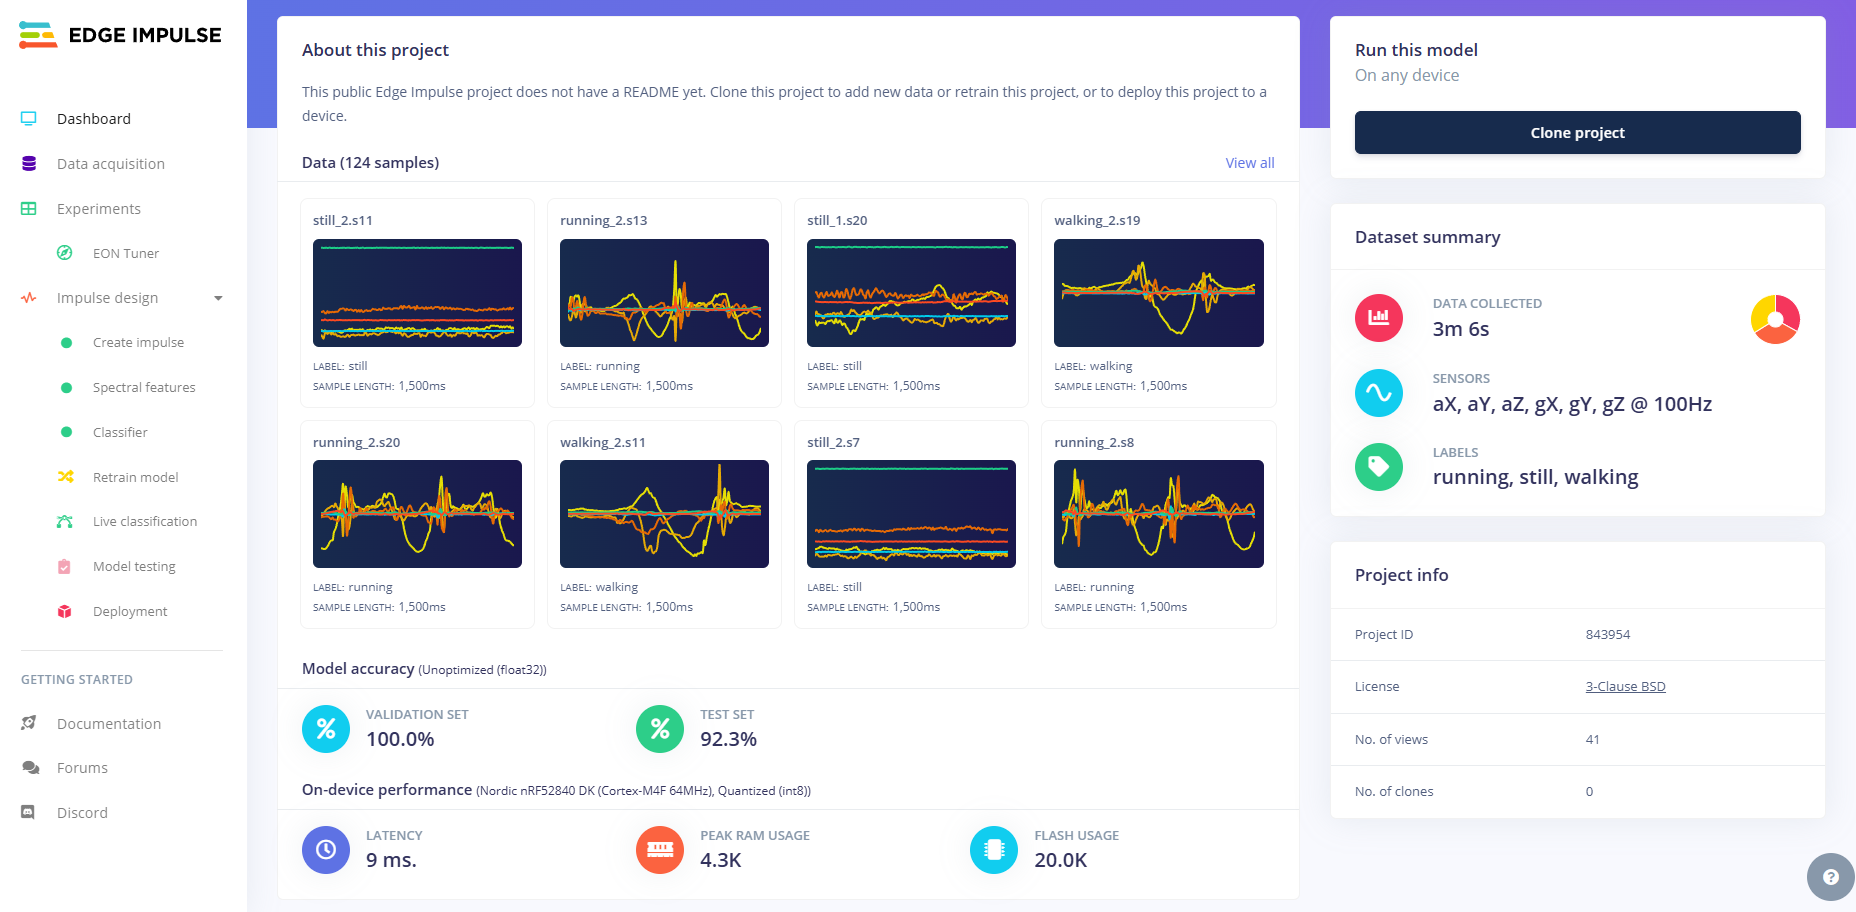
\includegraphics[width=0.85\textwidth]{figures/edge_impulse_interface.png}
\caption{Giao diện Edge Impulse (trang thiết kế Impulse): quy trình được định nghĩa bằng các block cố định, giới hạn khả năng tùy chỉnh tiền xử lý và thuật toán}
\label{fig:edge_impulse_ui}
\end{figure}

\subsection{Phân tích các nền tảng chính}

\paragraph{Edge Impulse \cite{web:Edge_Impulse}.} Nền tảng đám mây phổ biến nhất cho TinyML với EON Compiler tối ưu mã đầu ra và hỗ trợ 85+ mục tiêu vi điều khiển. Tuy nhiên, tiền xử lý bị cố định sau khi tải dữ liệu lên, không hỗ trợ phân đoạn tương tác; thuật toán chủ yếu giới hạn ở neural network; mã sinh ra là hộp đen không thể kiểm tra logic trích xuất đặc trưng; và dữ liệu phải lưu trên server của hãng, không phù hợp cho dữ liệu y tế nhạy cảm.

\paragraph{SensiML Analytics Toolkit \cite{web:SensiML}.} Hỗ trợ AutoML với hàng trăm đặc trưng ứng viên và Knowledge Packs cho MCU cụ thể. Hạn chế chính là chi phí rất cao, định dạng độc quyền, và lựa chọn đặc trưng theo kiểu hộp đen không giải thích được.

\paragraph{TensorFlow Lite Micro \cite{david2020tensorflow}.} Framework mã nguồn mở cung cấp runtime cho mạng nơ-ron lượng tử hóa trên MCU, tích hợp CMSIS-NN cho ARM và hỗ trợ INT8 quantization. Tuy nhiên, TFLite Micro chỉ hỗ trợ deep learning --- không triển khai được Random Forest hay SVM; không có công cụ tiền xử lý hay trích xuất đặc trưng; và interpreter runtime chiếm lượng flash đáng kể, đòi hỏi người dùng tự xây dựng toàn bộ pipeline từ đầu.

\paragraph{Teachable Machine (Google).} Giao diện no-code phù hợp cho tạo mẫu và giáo dục, nhưng thiếu trích xuất đặc trưng nâng cao, phân đoạn chuỗi thời gian, và chỉ xuất TensorFlow.js --- không chạy trên MCU.

\subsection{Tổng hợp khoảng trống}

Bảng~\ref{tab:platform_comparison} tổng hợp so sánh giữa các nền tảng và framework đề xuất.

\begin{table}[H]
\centering
\caption{So sánh các nền tảng Edge ML cho nhận dạng hoạt động}
\label{tab:platform_comparison}
\resizebox{\textwidth}{!}{%
\begin{tabular}{@{}p{4.0cm}p{3.2cm}p{3.2cm}p{3.2cm}p{4.4cm}@{}}
\toprule
\textbf{Tiêu chí} & \textbf{Edge Impulse} & \textbf{SensiML} & \textbf{TFLite Micro} & \textbf{Framework đề xuất} \\
\midrule
Chi phí & \$20--99/tháng & \$99--500/tháng & Miễn phí & Miễn phí (mã nguồn mở) \\
\midrule
Tiền xử lý tương tác & Hạn chế & Có (analytics) & Không & Có (kéo thả trên biểu đồ) \\
\midrule
Thuật toán & NN, transfer & RF, SVM, NN & Chỉ NN & RF, SVM, MLP, CNN \\
\midrule
Tạo mã & C++ (Arduino, ARM) & C (MCU cụ thể) & C++ (runtime) & C/C++/MicroPython đa đích \\
\midrule
Tối ưu hóa & Auto (EON) & AutoML & Lượng tử hóa & 4 chế độ rõ ràng \\
\midrule
Kiểm soát dữ liệu & Đám mây & Local/cloud & Local & Local hoàn toàn \\
\midrule
Xác minh tương đồng & Không minh bạch & Không & Không & Có (tự động) \\
\bottomrule
\end{tabular}%
}%
\end{table}

Điểm chung của các nền tảng hiện có: thiếu giao diện phân đoạn dữ liệu tương tác, bị giới hạn thuật toán hoặc chi phí cao, và sinh mã cho số ít nền tảng đích cố định. Đặc biệt, không nền tảng nào cung cấp cơ chế \textbf{xác minh tương đồng huấn luyện--triển khai} minh bạch. Khoảng trống này đặc biệt quan trọng trong bối cảnh nghiên cứu và giáo dục, nơi nhà nghiên cứu cần hiểu rõ pipeline, và các dự án nhỏ không có ngân sách cho giấy phép thương mại. \textbf{Luận văn này giải quyết khoảng trống đó} bằng một framework mã nguồn mở, minh bạch, hỗ trợ đa thuật toán và đa thiết bị.

\section{Phát biểu bài toán và mục tiêu nghiên cứu}
\label{sec:intro_problem}

\subsection{Phát biểu bài toán}

Từ các phân tích trên, bài toán nghiên cứu được phát biểu như sau:

\begin{quote}
\textit{Thiết kế và hiện thực một framework mã nguồn mở cho phép người dùng thực hiện toàn bộ quy trình HAR dựa trên cảm biến IMU --- từ thu thập dữ liệu, tiền xử lý tương tác, trích xuất đặc trưng, huấn luyện mô hình đa thuật toán, đến tự động sinh mã triển khai tối ưu cho nhiều họ vi điều khiển --- đồng thời đảm bảo tương đồng giữa kết quả huấn luyện và kết quả suy luận trên thiết bị biên.}
\end{quote}

Bài toán này đòi hỏi giải quyết đồng thời bốn thách thức: (1) hạ thấp rào cản kỹ thuật để người dùng không chuyên về nhúng vẫn triển khai được; (2) hỗ trợ nhiều thuật toán ML phù hợp cho tập dữ liệu nhỏ đến lớn; (3) sinh mã cho hệ sinh thái thiết bị phân mảnh; và (4) đảm bảo tính minh bạch và khả năng xác minh mã đã sinh.

\subsection{Mục tiêu nghiên cứu}

\begin{enumerate}
\item \textbf{Giao diện tiền xử lý tương tác}: Phát triển cơ chế phân đoạn và gán nhãn dữ liệu cảm biến trực tiếp trên biểu đồ tín hiệu bằng kéo thả, giảm thời gian chuẩn bị dữ liệu so với viết mã thủ công.

\item \textbf{Hỗ trợ đa thuật toán với giao diện thống nhất}: Tích hợp Random Forest, SVM, MLP, CNN với giao diện huấn luyện chung, cho phép so sánh và chọn mô hình phù hợp với từng ràng buộc phần cứng.

\item \textbf{Kiến trúc sinh mã đa đích}: Thiết kế hệ thống sinh mã phân lớp ánh xạ cùng một mô hình sang nhiều họ thiết bị (Arduino, ARM Cortex-M, ESP-IDF, Zephyr, MicroPython) với bốn chế độ tối ưu hóa (accuracy, speed, power, balanced).

\item \textbf{Đảm bảo tương đồng huấn luyện--triển khai}: Xây dựng cơ chế xác minh mã C++ sinh ra tái tạo chính xác công thức trích xuất đặc trưng, tham số chuẩn hóa, thứ tự đặc trưng và trọng số mô hình, đảm bảo nhất quán kết quả suy luận giữa Python và MCU.

\item \textbf{Xác thực trên phần cứng thực}: Đánh giá framework trên thiết bị ARM Cortex-M4F với dữ liệu HAR thực tế, đo thời gian suy luận, mức sử dụng bộ nhớ, và so sánh trực tiếp với nền tảng thương mại Edge Impulse.
\end{enumerate}

\subsection{Đóng góp chính}

Nghiên cứu này đóng góp vào lĩnh vực Edge ML và nhận dạng hoạt động qua các điểm mới sau:

\begin{enumerate}
    \item \textbf{Framework tích hợp toàn diện}: Lần đầu tiên kết hợp tiền xử lý tương tác (kéo thả trên biểu đồ), trích xuất đặc trưng minh bạch, huấn luyện đa thuật toán, và sinh mã đa đích trong cùng một hệ thống mã nguồn mở.
    
    \item \textbf{Cơ chế xác minh tương đồng huấn luyện--triển khai}: Quy trình kiểm tra 12 điểm đảm bảo mã C++ sinh ra tái tạo chính xác kết quả Python --- giải quyết vấn đề training--deployment gap mà các nền tảng hiện có bỏ qua.
    
    \item \textbf{Kiến trúc sinh mã đa chiều}: Mô hình Factory Pattern ánh xạ ba trục (loại mô hình × nền tảng đích × backend triển khai), cho phép một mô hình đã huấn luyện xuất đồng thời sang nhiều họ thiết bị mà không cần huấn luyện lại.
    
    \item \textbf{Phát hiện kỹ thuật mới}: Tài liệu hóa các lỗi tương đồng chưa được báo cáo trong tài liệu (zero-padding artifact, sai lệch population vs sample std trong kurtosis, feature order mismatch) --- kiến thức có giá trị cho cộng đồng TinyML.
    
    \item \textbf{Kết quả thực nghiệm}: Đạt 97--99\% trên bài toán 5 lớp, vượt trội Edge Impulse trên cùng tập dữ liệu (F1=1,00 vs 0,96), với mức sử dụng flash nhỏ hơn đáng kể (18--23\% vs 51\%) và thời gian suy luận 20~ms.
\end{enumerate}

Hình~\ref{fig:workflow} tổng hợp quy trình làm việc hoàn chỉnh mà framework cung cấp.

\begin{figure}[H]
\centering
\resizebox{\linewidth}{!}{%
\begin{tikzpicture}[
    node distance=0.55cm,
    stepbox/.style={
        rectangle, rounded corners=5pt,
        minimum width=2.6cm, minimum height=2.0cm,
        text width=2.5cm, align=center,
        draw=blue!45!black, fill=blue!6,
        line width=0.9pt, font=\small,
    },
    arr/.style={
        -{Stealth[length=7pt, width=5pt]},
        line width=2pt, color=black!35,
    },
    badge/.style={
        circle, fill=blue!65!black,
        minimum size=20pt, inner sep=0pt,
        font=\small\bfseries, text=white,
    },
    phaselbl/.style={
        font=\small\bfseries, text=black!65,
    },
    timelbl/.style={
        font=\scriptsize\itshape, text=black!45,
    },
]
    % --- Step boxes ---
    \node[stepbox] (s1) {\textbf{Dữ liệu}\\[4pt]\scriptsize Tải file CSV};
    \node[stepbox, right=of s1] (s2) {\textbf{Tiền xử lý}\\[4pt]\scriptsize Lọc \& phân đoạn};
    \node[stepbox, right=of s2] (s3) {\textbf{Đặc trưng}\\[4pt]\scriptsize Cửa sổ kéo thả};
    \node[stepbox, right=of s3] (s4) {\textbf{Huấn luyện}\\[4pt]\scriptsize RF / SVM / NN};
    \node[stepbox, right=of s4] (s5) {\textbf{Tạo mã}\\[4pt]\scriptsize C++ / Python};
    \node[stepbox, right=of s5] (s6) {\textbf{Thiết bị}\\[4pt]\scriptsize Triển khai biên};

    % --- Phase grouping backgrounds ---
    \begin{scope}[on background layer]
        \node[rectangle, rounded corners=8pt,
              fill=blue!10, draw=blue!30!black,
              inner sep=8pt, line width=0.8pt,
              fit=(s1)(s2)] (ph1) {};
        \node[rectangle, rounded corners=8pt,
              fill=teal!10, draw=teal!30!black,
              inner sep=8pt, line width=0.8pt,
              fit=(s3)(s4)] (ph2) {};
        \node[rectangle, rounded corners=8pt,
              fill=orange!10, draw=orange!30!black,
              inner sep=8pt, line width=0.8pt,
              fit=(s5)(s6)] (ph3) {};
    \end{scope}

    % --- Phase labels above groups ---
    \node[phaselbl, above=0.5cm of ph1] {Thu thập \& Xử lý};
    \node[phaselbl, above=0.5cm of ph2] {Xây dựng Mô hình};
    \node[phaselbl, above=0.5cm of ph3] {Triển khai Biên};

    % --- Arrows between steps ---
    \foreach \a/\b in {s1/s2, s2/s3, s3/s4, s4/s5, s5/s6}
        \draw[arr] (\a) -- (\b);

    % --- Step number badges centred on top border ---
    \foreach \n/\i in {s1/1, s2/2, s3/3, s4/4, s5/5, s6/6}
        \node[badge] at (\n.north) {\i};

    % --- Time labels below ---
    \node[timelbl, below=0.3cm of s1] {$\sim$5 phút};
    \node[timelbl, below=0.3cm of s2] {$\sim$10 phút};
    \node[timelbl, below=0.3cm of s3] {$\sim$2 phút};
    \node[timelbl, below=0.3cm of s4] {5--30 phút};
    \node[timelbl, below=0.3cm of s5] {$\sim$1 phút};
    \node[timelbl, below=0.3cm of s6] {$\sim$5 phút};
\end{tikzpicture}%
}
\caption{Quy trình làm việc từ dữ liệu thô đến triển khai biên (tổng ước tính 30--60 phút)}
\label{fig:workflow}
\end{figure}

\section{Phạm vi nghiên cứu}

Nghiên cứu tập trung vào HAR dựa trên IMU 6 trục (gia tốc kế + con quay hồi chuyển), sử dụng các thuật toán học máy có giám sát. Đánh giá phần cứng định lượng tập trung trên nền tảng tham chiếu Seeed XIAO nRF52840 (ARM Cortex-M4F, 64~MHz, 256~KB RAM); các nền tảng đích còn lại (ESP-IDF, Zephyr, MicroPython) được phân tích ở mức sinh mã và khả năng biên dịch.

Nghiên cứu không bao gồm: hợp nhất cảm biến đa phương thức (camera, âm thanh); nhập mô hình từ framework bên ngoài (TensorFlow SavedModel, ONNX); cập nhật mô hình trên thiết bị (on-device learning); và ứng dụng y tế đòi hỏi chứng nhận lâm sàng.

\section{Tổ chức luận văn}

Luận văn gồm sáu chương. \textbf{Chương~\ref{chap:relatedwork}} đánh giá các công trình liên quan về hệ thống HAR, framework học máy cho thiết bị biên, và các nền tảng triển khai edge ML hiện có. \textbf{Chương~\ref{chap:methodology}} trình bày phương pháp luận: quy trình tiền xử lý tín hiệu, các phương pháp trích xuất đặc trưng (miền thời gian, miền tần số, bất biến hướng), huấn luyện đa thuật toán, và chiến lược sinh mã đảm bảo tương đồng huấn luyện--triển khai. \textbf{Chương~\ref{chap:design_implementation}} mô tả thiết kế và hiện thực hệ thống, bao gồm kiến trúc phần mềm, giao diện người dùng và chi tiết triển khai các module. \textbf{Chương~\ref{chap:results}} báo cáo kết quả thực nghiệm: hiệu suất phân loại của năm thuật toán trên bài toán 3 và 5 lớp, đặc điểm triển khai trên thiết bị thực (thời gian suy luận, mức sử dụng bộ nhớ), và so sánh trực tiếp với Edge Impulse. \textbf{Chương~\ref{chap:discussion_conclusion}} trình bày kết luận, thảo luận các phát hiện chính, hạn chế và hướng phát triển tương lai.
